%%%%%%%%%%%%%%%%%%%%%%%%%%%%%%
\chapter{Background}

In this chapter, details regarding the simulation theory are gone over.  

%%%%%%%%%%%%%%%%%%%%%%%%%%%%%%
\section{Reactor Analysis}

reactors in general, LWR, fast breeders, GenIV, waste streams, power conversion

fission chain reaction, 7 factor formula?

coupling between TH, need for fast simulations in oder to do convergence iterations




%%%%%%%%%%%%%%%%%%%%%%%%%%%%%%
\subsection{History}

The Monte Carlo method is not a new way to simulate nuclear reactors (or any particle transport problem for that matter) and in it's modern form dates back to 1940 when XXX invented the approach while working on the Manhattan Project[cite]. Uncle in Monaco...  During this time, Henry Metropolis and John Von Neumann...[cite]  Although this may be disputed by some people since is was rumored that Enrico Fermi was basically doing small scale simulations of this kind in his head trying to get the Chicago Pile critical [cite].


%%%%%%%%%%%%%%%%%%%%%%%%%%%%%%
\subsection{Nuclear Data}

it's all about the data, complexity?

endf

measurements?

heirarchy




%%%%%%%%%%%%%%%%%%%%%%%%%%%%%%
\subsection{Nuclear Interactions}

The core of a Monte Carlo simulation is explicitly modeling the individual interactions the neutron undergoes as it moves through matter.  At the highest level, these reactions can be broken down into two categories, elastic reactions and inelastic reactions.  Elastic reactions are those where both momentum and kinetic energy are conserved, i.e. ones where any energy the neutron loses is given to the target nucleus.  Inelastic reactions are those that conserve momentum but do not conserve kinetic energy, i.e. ones where the kinetic energy of the particles can be converted to a vibrational mode of the target nucleus, etc.  These reactions are further divided by the number and type of secondary particles they produce.  Reactions that produce no secondary neutrons are called ``disappearance'' reactions since the neutron effectively disappears, reactions that produce a single neutron are typically called scattering reactions since they effectively change the incoming neutron's energy and direction, and reaction the produce more than one particle are simply called ``secondary-producing'' reactions. Table \ref{nuc_reaction_summary} show a summary of the reaction classifications, and it can be seen that elastic scattering is the only elastic reaction.   

potential scattering vs compound nucleus.

\begin{table}[h]
\centering
\caption{Summary matrix of how neutron reactions are classified.}
\label{nuc_reaction_summary}
\begin{tabular}{| l | c | c | c |}
\multicolumn{4}{c}{Number of Secondaries} \\
\hline
  & 0 & 1 & $>$1 \\
 \hline
 Elastic & & Elastic Scatter & \\
 \hline
 Inelastic & Disappearance & Inelastic Scatter & Secondary-Producing \\
\hline
\end{tabular}
\end{table}

The probabilities for individual reactions occurring are expressed in terms of cross sections.  In simple terms, nuclear cross sections are like a geometric cross sections -they represent the ``size'' of the target nucleus for a particular reaction.  The classical analogy is that if neutrons and nuclei are hard spheres, and neutrons are randomly shot through a material, more neutrons will hit the larger targets than the smaller ones.  Cross sections are also expressed in units of area, the ``barn,'' which is $10^{-24}$ cm$^2$.  This unit was coined by Baker and Holloway while performing scattering experiments with uranium since ``a cross section of $10^{-24}$ cm$^2$ for nuclear purposes was really as big as a barn''\cite{LAMS523}.  Of course, nuclear cross sections have no literal meaning in terms of the actual sizes of the nuclei, they only represent the likelihood of a particular reaction occurring.  Working from the macroscopic scale, which is where measurements are taken, a \emph{macroscopic cross section}, represented by greek capital sigma ($\Sigma$), is the probability of a reaction happening within an infinitesimal distance d$x$.  With this parameter, we can write down an equation that describes the survival probability of a group of particles.  Describing a group is necessary since the dimension x is \emph{continuous}.  Given a particle packet containing N particles and $\Sigma$, their interaction probability over $d$x, the change the population over $d$x is the product of the population N and the interaction probability, as show in \eqref{pop_diff}.

\begin{equation}
\frac{d\mathrm{N}}{d\mathrm{x}} = - \Sigma \mathrm{N}
\label{pop_diff}
\end{equation}

Integrating \ref{pop_diff} over an interval yields an expression for the number of \emph{non-interacting} particles left in a packet after crossing that interval.  Dividing the surviving number by the initial gives a dimensionless expression for the non-interaction probability, P$_\mathrm{NI}$, over the interval x$_1$ as shown in \eqref{pop_NI}.

\begin{equation}
\mathrm{P}_\mathrm{NI} = \frac{\mathrm{N}}{\mathrm{N}_0} = \mathrm{e}^{- \Sigma \mathrm{x}_1}
\label{pop_NI}
\end{equation}

\begin{equation}
\Sigma = \frac{ - \mathrm{ln}(    \mathrm{I} / \mathrm{I}_0  )  }  {\mathrm{x}_1}
\label{pop_beam}
\end{equation}

Since these expressions also apply to beam intensity, they can be used to measure the cross sections for materials by rearranging the equations into the form shown in \eqref{pop_beam}.  If the source intensity, the exiting intensity, and the material thickness are all known, the macroscopic cross section for that material can be determined.  On a microscopic level, however, the neutron interaction probabilities only depend on the type of nucleus, not the aggregate material.  To correct for this, the measured macroscopic cross section can be divided by the number density of nuclei in the material to give the microscopic cross section, $\sigma$, which is material-independent and only depends on the isotope.  In \eqref{micro_exp}, N represents the number density in units of cm$^{-3}$, $\rho$ represents the material density in terms of g*cm$^{-3}$, and M represents the nuclear mass in g.  The microscopic cross section has units of barns, and is what is given in nuclear data files.  They are more general since they are not material-dependent and can be summed into a total material macroscopic cross section by weighting individual microscopic cross sections with the number density of an isotope in a material, as show in \eqref{material_sum_xs}.  In this expression, $f_\mathrm{i}$ is the atomic fraction of isotope i in the material.


\begin{equation}
\Sigma = N \sigma = \frac{\rho}{M} \sigma
\label{micro_exp}
\end{equation}

\begin{equation}
\sum_{\mathrm{i}=1}^{\mathrm{N}_\mathrm{isotopes}} f_\mathrm{i} =1
\label{fraction_norm}
\end{equation}

\begin{equation}
\Sigma_{\mathrm{material}} = \mathrm{N}_1 \sigma_1 +  \mathrm{N}_2 \sigma_2 + \mathrm{N}_3 \sigma_3+ ... = \sum_{\mathrm{i}=1}^{\mathrm{N}_\mathrm{isotopes}} \mathrm{N}_\mathrm{i} \sigma_\mathrm{i} = \rho\frac{\sum_{\mathrm{i}=1}^{\mathrm{N}_\mathrm{isotopes}} f_\mathrm{i}\sigma_\mathrm{i} } { \sum_{\mathrm{i}=1}^{\mathrm{N}_\mathrm{isotopes}} f_\mathrm{i} \mathrm{M}_\mathrm{i}}
\label{material_sum_xs}
\end{equation}

The above expressions do not take energy into account, so they are assumed to be at a single energy.  Using such simple expressions to determine the cross section of an isotope would only be valid with the use of a very, very precisely mono-energetic beam.  The quantum mechanical details that go into cross sections can cause them to depend strongly on the energy (or velocity) of the neutron and the target nucleus.  Many nuclides have resonances where the interactions probability spikes to very large values.  This typically happens when the incoming energy is exactly that of an energy level of the resultant compound nucleus \cite{duderstadt}.   Figure \ref{xs_e_dependence_li} shows the energy dependence of various reactions type in lithium-6 and Figure \ref{xs_e_dependence_u} shows the dependence of others in uranium-235.  

\begin{figure}[h!]
  \label{xs_e_dependence_li}
  \centering
    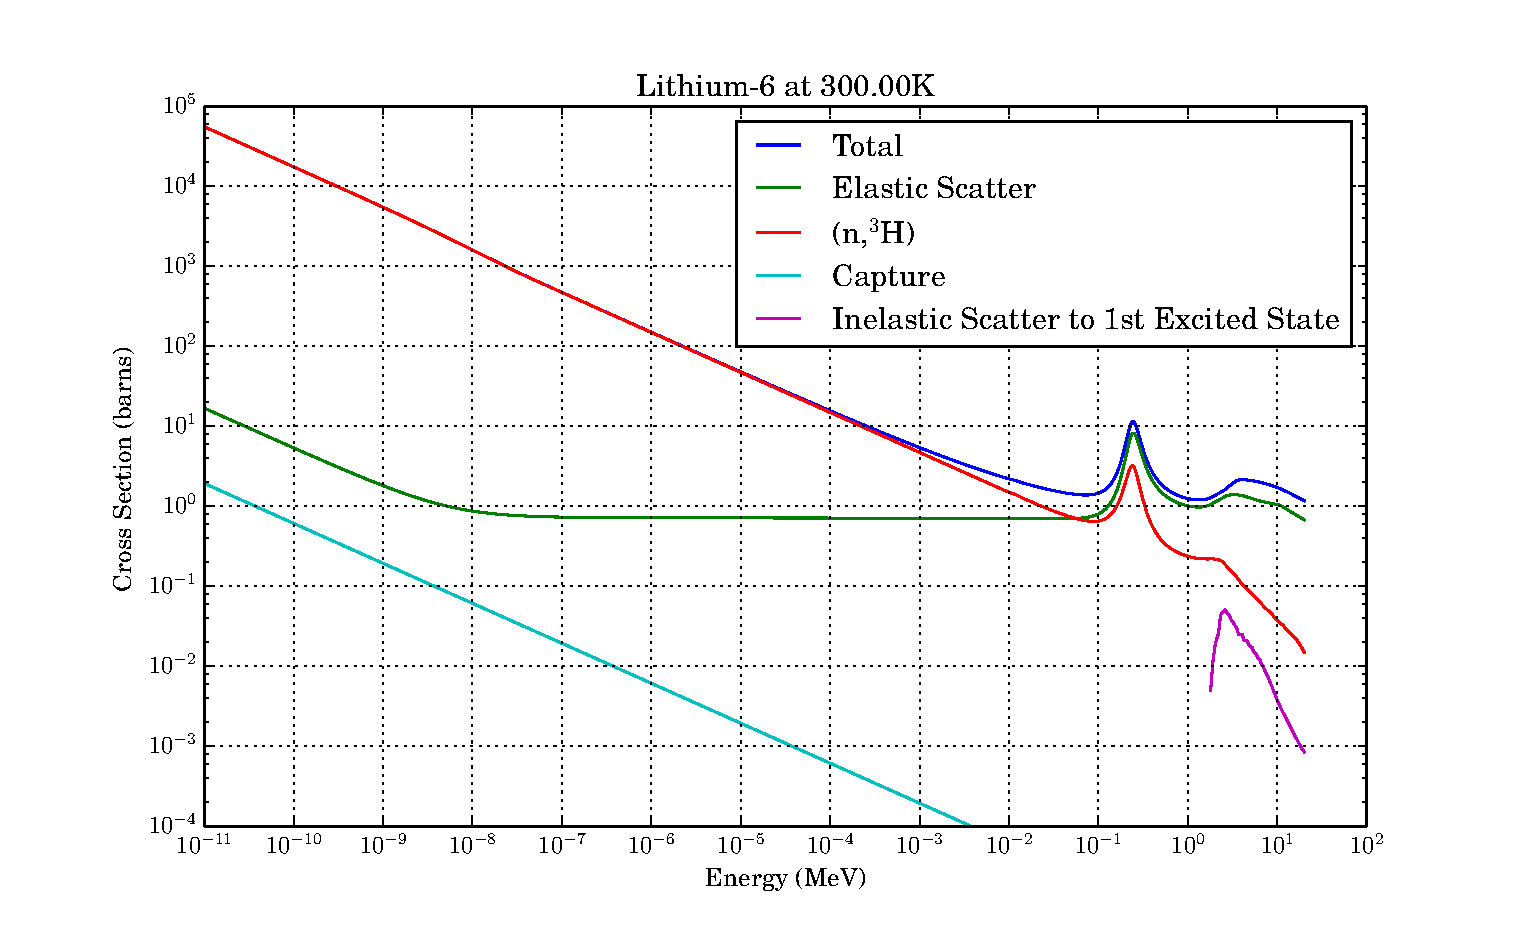
\includegraphics[width=0.8\textwidth]{graphics/xs_li6.eps}
     \caption{The energy dependence of some reactions in lithium-6.}
\end{figure}

\begin{figure}[h!]
  \label{xs_e_dependence_u}
  \centering
    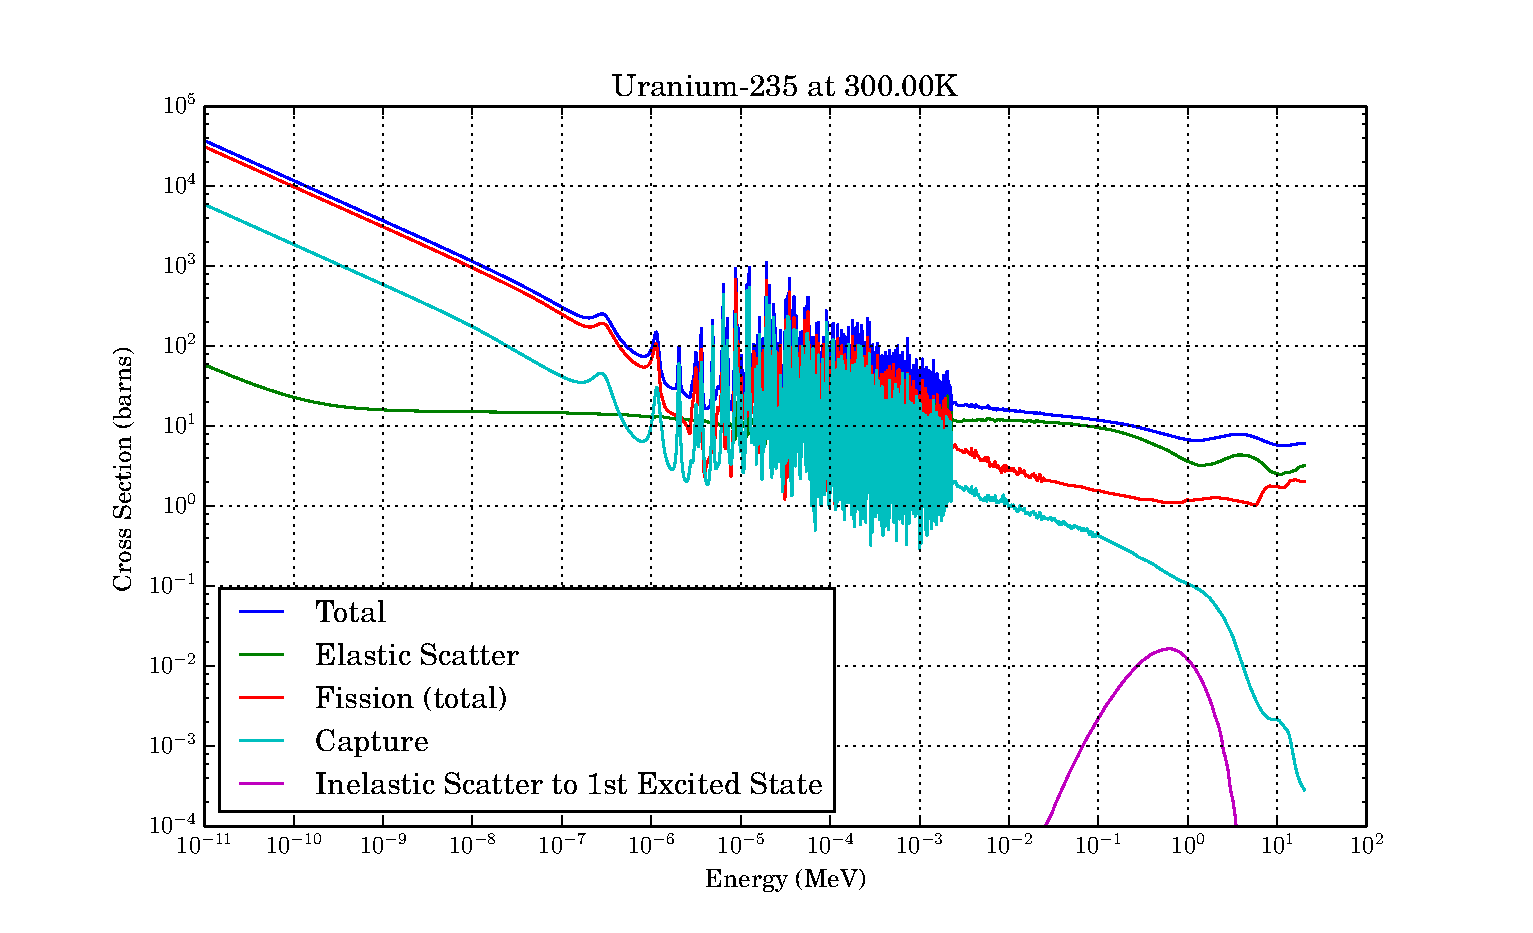
\includegraphics[width=0.8\textwidth]{graphics/xs_u235.eps}
    \caption{The energy dependence of some reactions in uranium-235.}
\end{figure}

It is important to note the complexity shown in uranium-235 in the 0.1eV to 40keV range.  This is referred to as the ``resonance region'' and adds much of the complexity in accurately modeling neutron transport.  There are no simple functional representations available for these types of cross sections, so they must be represented in a point-wise tabular format.  It is also important to note that at low energies, cross sections typically lose structure and exhibit the same ``1/$v$'' scaling.  This is due to the particle and the target having more time to interact with each other.  The energy levels where this phenomenon exists is similar the thermal energy of the target and the target no longer appears stationary from the neutrons perspective.  If the neutron is slow enough, the targets appear to be moving instead of the neutron, and more of them come into the neutrons sphere of interaction.  This is the qualitative reason for 1/$v$ scaling at low energies.  Due to to their identical scaling, the ratios between the reaction types stays constant as velocity is decreased but the overall interaction probability with respect to distance increases.

In the next subsections, the characteristics and kinematics of the different reaction types are explained.

\subsubsection{Elastic Scattering}

Elastic scattering conserves both the momentum and the kinetic energy of the reacting particles and occurs when the neutron does not enter the nucleus, only bounces off of it's potential field.  Since there is only a single exiting particle, elastic scattering is a two-body interaction and the exiting energies can be determined if the angle between the exiting particle is known.  This problem is greatly simplified if the interacting particles' velocities are transformed into the center-of-mass (CM) frame, where net momentum is zero. The velocity of the CM is defined in \eqref{vCM} where $m$ and $M$ are the neutron's and the target's respective masses, $v$ and $V$ are their respective velocity vectors, and $A$ is the ratio of the target's mass to the neutron's mass (also know as the ``atomic weight ratio'' or AWR).  The derivation from here follows closely with that in ref \cite{jaakko}.

\begin{equation}
A = \frac{M}{m}
\label{AWR}
\end{equation}

\begin{equation}
\boldsymbol{v_{\mathrm{CM}}} = \frac{ m \boldsymbol{v} + M \boldsymbol{V} }    {m+M} = \frac{ \boldsymbol{v} + A \boldsymbol{V} }    {1+A}
\label{vCM}
\end{equation}

The CM velocities of the target and the neutron are then calculated by subtracting the CM velocity out of them, ash shown in \eqref{CM}.  The $_\mathrm{c}$ subscript will denote the CM-frame values from now on, whereas $v_{\mathrm{CM}}$ will denote the velocity of the CM frame relative to the lab frame.

\begin{equation}
\begin{split}
 \boldsymbol{v_{_\mathrm{c}}} &= \boldsymbol{v} - \boldsymbol{v_{\mathrm{CM}}} \\  
 \boldsymbol{V_{\mathrm{c}}} &= \boldsymbol{V} - \boldsymbol{v_{\mathrm{CM}}}
 \end{split}
\label{CM}
\end{equation}

Once in the CM frame, the equation for conservation of momentum can be written as \eqref{consMomCM}.  The primed values are those after the collision.  Since the net momentum is zero, the directions of the neutron and the target must be in opposite directions as shown in \eqref{rotationCM}.

\begin{equation}
\begin{split}
m \boldsymbol{v_{_\mathrm{c}}} + M \boldsymbol{V_{_\mathrm{c}}} &= m \boldsymbol{v_{_\mathrm{c}}^\prime} + M \boldsymbol{V_{_\mathrm{c}}^\prime} = 0\\
    \boldsymbol{v_{_\mathrm{c}}} + A  \boldsymbol{V_{_\mathrm{c}}} &=     \boldsymbol{v_{_\mathrm{c}}^\prime} + A  \boldsymbol{V_{_\mathrm{c}}^\prime} = 0
\end{split}
\label{consMomCM}
\end{equation}

\begin{equation}
\begin{split}
\boldsymbol{v_{_\mathrm{c}}^\prime} &= - A  \boldsymbol{V_{_\mathrm{c}}^\prime} \\
\boldsymbol{v_{_\mathrm{c}}} &= -A  \boldsymbol{V_{_\mathrm{c}}}
\end{split}
\label{rotationCM}
\end{equation}

The equation for conservation of energy is shown in \ref{consECM}.  Energy is a scalar quantity, and therefore these equations are as well.  There are no vectors, which are indicated with boldface type, since $v^2 =( \boldsymbol{v} \cdot \boldsymbol{v})$.  $Q$ is the amount of energy released by the reaction, and is zero here but is convenient to include in this derivation for use in inelastic collision kinematics where it is nonzero.

\begin{equation}
\begin{split}
m v_{_\mathrm{c}}^2 + M V_{_\mathrm{c}}^2 &= m v_{_\mathrm{c}}^{\prime2} + M V_{_\mathrm{c}}^{\prime2} + 2Q \\
    v_{_\mathrm{c}}^2 + A  V_{_\mathrm{c}}^2 &=     v_{_\mathrm{c}}^{\prime2} + A  V_{_\mathrm{c}}^{\prime2} + \frac{2Q}{m}
\end{split}
\label{consECM}
\end{equation}

There are now two unknowns (the primed values) and two equations, and the final velocities of the neutron and the target can be determined.  Substituting \eqref{rotationCM} into \eqref{consECM} and solving yields either equation in \eqref{finalvCM}, depending on how the substitution is done.  It can be seen that if $Q$ is zero, as it is in elastic scattering, the initial and final velocities are the same for the particles and the interaction only causes a rotation in the CM frame.

\begin{equation}
\begin{split}
v_{_\mathrm{c}}^{\prime} &=  \sqrt{ v_{_\mathrm{c}}^{2} + \frac{2AQ}{m(A+1)}  }  \\
V_{_\mathrm{c}}^{\prime} &= \sqrt{ V_{_\mathrm{c}}^{2} + \frac{2Q}{mA(A+1)}  } 
\end{split}
\label{finalvCM}
\end{equation}

At first glance, it seems like the interaction has been fully characterized, but \eqref{rotationCM} only relates the initial states of the neutron and the target to one another and the final states of neutron and the target to one another.  The initial state and final state of the neutron still need to be related.  It has been mentioned already that the interaction is only a rotation in the CM frame, so the initial and final state of the neutron's direction can be related by a three-dimensional rotation formula.  An efficient algorithm is given by the Rodrigues' rotation formula, shown in \eqref{RodriguesRot}.  In the formula, $\boldsymbol{k}$ is an auxilliary unit vector around which $\boldsymbol{v}$ is being rotated.  From this unit vector, $theta$ is the angle $\boldsymbol{v}$ is rotated away from $\boldsymbol{k}$ such that $(\boldsymbol{v} \cdot \boldsymbol{v_{\mathrm{rot}}}) = |v||v_{\mathrm{rot}}|\cos\theta$.  It is ``efficient'' in the sense that to rotate a vector, a full 3x3 matrix does not need to be constructed and multiplied by the vector. In other words, matrix-vector operations are not needed and it can be carried out with only vector operations \cite{}.

\begin{equation}
 \boldsymbol{ v_{ \mathrm{rot}}} = \boldsymbol{v} \cos \theta + (\boldsymbol{k} \times \boldsymbol{v}) \sin \theta + \boldsymbol{k} (\boldsymbol{k} \cdot \boldsymbol{v})(1-\cos \theta)
\label{RodriguesRot}
\end{equation}

If the polar and azimuthal rotation angles, $\theta$ and $\phi$, respectively, are determined, the initial neutron velocity vector can be rotated through these angles to its final value.  After the rotation is done, the final velocities are known in the CM frame and they can be transformed back to the lab frame to give the final velocities there, as shown in \eqref{xformbackCM}.

\begin{equation}
\begin{split}
 \boldsymbol{v^{\prime}}  &= \boldsymbol{v_{\mathrm{c}}^{\prime}} + \boldsymbol{v_{\mathrm{CM}}} \\  
 \boldsymbol{V^{\prime}} &= \boldsymbol{V_{\mathrm{c}}^{\prime}} + \boldsymbol{v_{\mathrm{CM}}}
 \end{split}
\label{xformbackCM}
\end{equation}


\subsubsection{Inelastic Level Scattering}

Inelastic scattering is the other type of scattering a neutron can undergo where kinetic energy is no longer conserved.  An amount of energy is either released from the reaction to the particles, or more commonly, taken from the particles and lost to the reaction.  In neutron-nucleus collisions, the target nucleus can be excited to a higher energy state than its ground state if the colliding neutron has a high enough energy to do so.  If it does and the collision excites the nucleus, a discrete amount of energy equal to the energy of the excited state is lost to the reaction.  These excited states typically do not have long half lives, and a gamma ray is emitted when the nucleus relaxes to its ground state.  This type of reaction is called inelastic level scattering due to a an excited energy \emph{level} becoming occupied by the target nucleus.  

Since it is still a two-body interaction, the kinematics of the reaction are identical to elastic scattering except the $Q$ value is nonzero and negative.  These reactions have a threshold energy below which their cross sections are zero since the neutron would not have enough energy to excite the state.   Figure \ref{Elevels} shows the energy levels in lead-XXX, which is often used as a fast neutron moderators due to its many, low-lying energy levels and its large inelastic scattering cross sections.

\begin{figure}[h!]
  \label{Elevels}
  \centering
    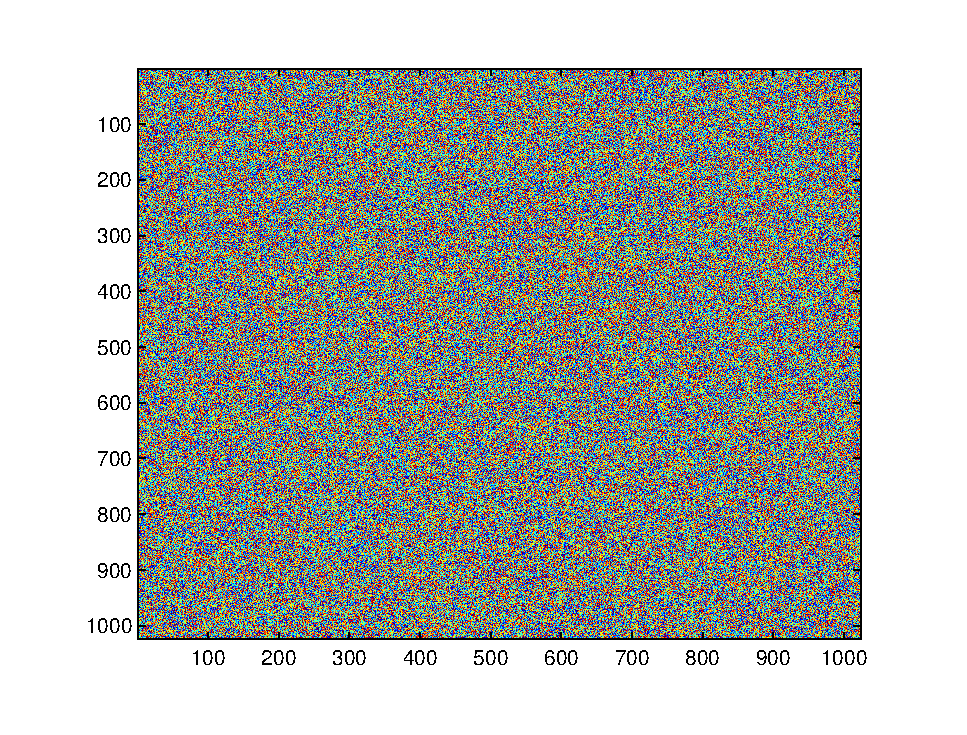
\includegraphics[width=0.8\textwidth]{graphics/noise.eps}
     \caption{The energy levels of lead-XXX\cite{}.}
\end{figure}

\subsubsection{Inelastic Continuum Scattering}

At energies above the distinct levels there lies a continuum in the nuclear energy states.  This isn't truly a ``continuum'' in the strictest sense, but the energy levels become so close together they they effectively form a domain where energy can take continuous values.  Unlike the discrete $Q$ values corresponding to a single excited state used in inelastic level scattering, the $Q$ value of the reaction now follows a distribution.

\subsubsection{Disappearance Reactions}

Unlike scattering reactions, where the energy and direction of the neutron is changed but continues to transport, \emph{disappearance} reactions remove a free neutron.  Typically this \emph{capture} of a neutron leaves the daughter nucleus in an excited state, which them relaxes to ground state by emitting a gamma ray.


\subsubsection{Fission}

Fission means ``the splitting splitting of something into two parts'' in the literal sense of the word.  This is exactly what nuclear fission is as well.  It is when a nucleus splits into two smaller nuclei, called \emph{fission fragments}.  When heavy nuclei undergo fission, they release energy, and typically emit a few other particles, including neutrons.  That this reaction releases energy is the reason heavy elements, like uranium, can be used as an energy source.  This is because the fission fragments have a higher binding energy per nucleon compared to the parent nucleus.  Figure \ref{binding_e_per_nuc} shows the average binding energy per nucleon for a wide range of isotopes.  Note that the peak of the curve is at Iron-56, the most tightly bound nucleus, and that heavier nuclides are lower than it.  Fission splits the parent into two lighter nuclides, and since the fragments are more tightly bound, the excess binding energy from the parent is released.  The released energy isn't simply deposited as heat directly, however, it is released in a range of forms.  Fission doesn't just release some energy, it releases a substantial amount of it.  Uranium-235, for example, releases a total of 192.9$\pm$0.5 \emph{MeV} per fission \cite{duderstadt}.  Compared to chemical energy sources where the energy released per reaction is on the order of 1\emph{eV}.  Fission energy yield is 8 orders of magnitude larger!  Not all of this energy is converted to heat, bit a substantial amount is.  Table \ref{fission_dist} shows the fraction of this total energy that is given to each entity.  Note that a significant fraction is given to neutrinos, which is essentially lost due to their very small interaction cross section.  The kinetic energy of the fission fragments has the majority of the energy, and since they are heavy and charged, their energy is deposited as heat very near to the fission site.  Other particles, light photons and neutrons, carry some of the fission energy further away from the fission site, but their energy mostly still ends up as heat.
  
\begin{figure}[h!]
\label{binding_e_per_nuc}
  \centering
    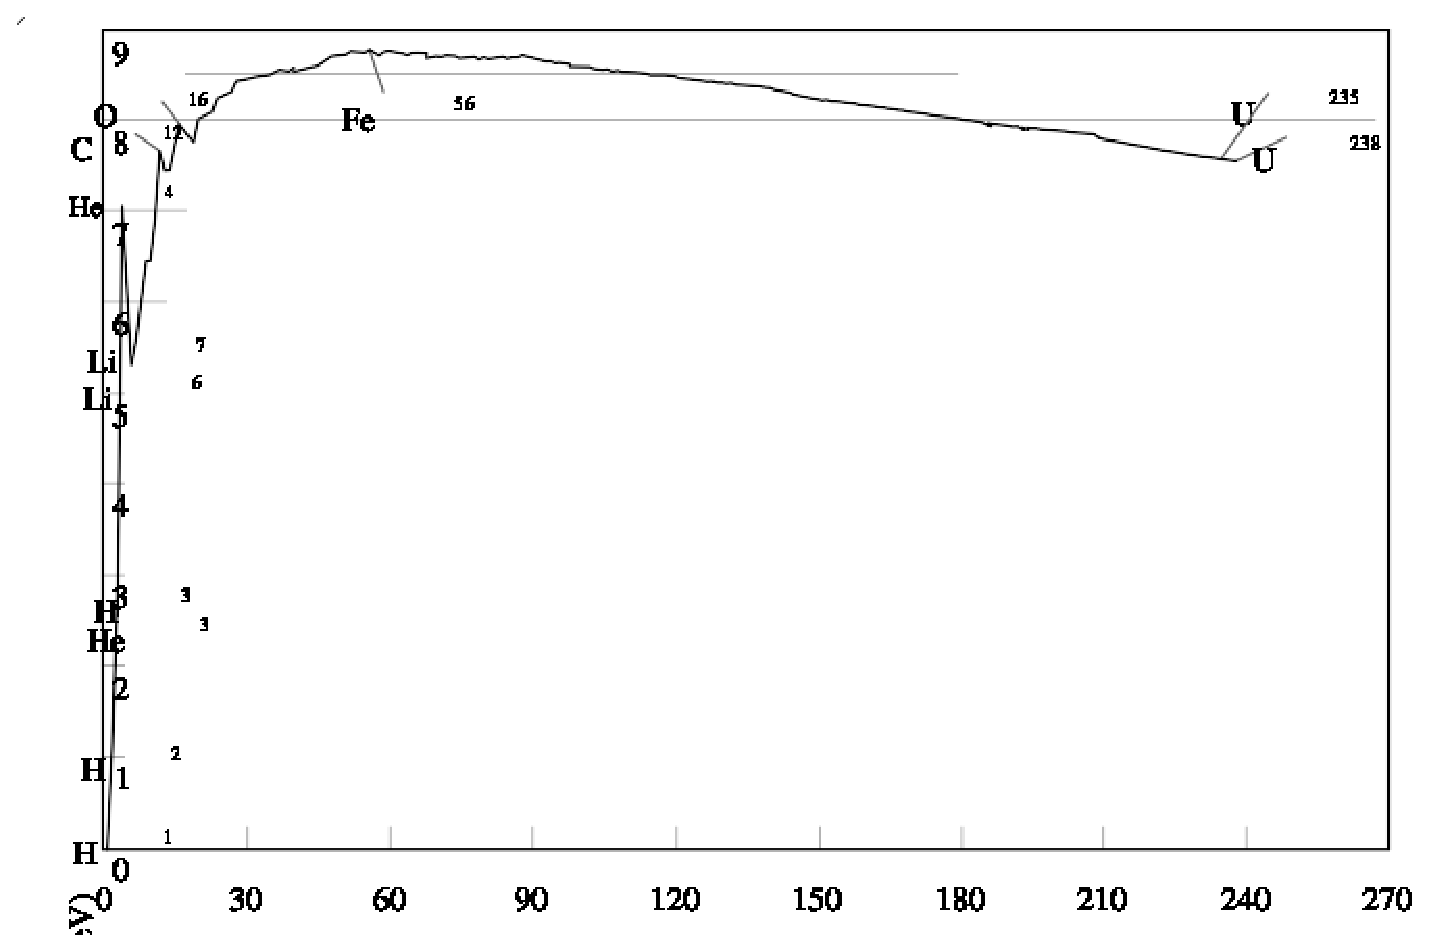
\includegraphics[width=0.8\textwidth]{graphics/binding_e_per_nuc.eps}
     \caption{Average binding energy per nucleon.  REPLACE ME WITH ONE YOU MAKE YOURSELF FROM DATA. \cite{}.}
\end{figure}

\begin{table}[h]
\centering
\caption{Average distribution of fission energy \cite{duderstadt}.}
\label{fission_dist}
\begin{tabular}{| l | c | r | r |}
\hline
Particle & Energy (\%) & Range & Time \\
\hline
Fission fragment kinetic energy & 80 & $<$0.1cm & prompt \\
\hline
Prompt neutrons & 3 & 10-100cm & prompt \\
\hline
Photons & 4 & 100cm & prompt \\
\hline
Fission product $\beta$ decay & 4 & short & delayed \\
\hline
Neutrinos &  5 & extremely long & delayed \\
\hline
Nonfission reactions from n capture & 4 & 100cm & delayed \\
\hline
\end{tabular}
\end{table}

Fission is technically considered a disappearance reaction as well since the fission-inducing neutron is absorbed by the nuclide.  Even though is is absorbed, more than 2 new neutrons are released by fission, enabling the fission chain reaction to occur.  An important parameter of the fission chain reaction is $nu$, the fission neutron yield.    The total yield is different than the prompt yield in that it also includes neutrons produced from photon-induced emission and from fission product decay.  These neutrons are not ``prompt'' in that they are not emitted immediately from the fission itself.  The processes that create these ``delayed'' neutrons (decay and nuclear relaxation) take time to occur.  Prompt neutrons appear immediately after fission, whereas delayed neutrons can appear anywhere between 0.6 to 80 seconds after.  The kinetics of a nuclear chain reaction depend heavily on the fraction the delayed neutrons which sustain the chain reaction.  Since they have a relatively large time delay, they cause the time between subsequent neutron generations to become longer.  This time between generations is called the \emph{effective neutron lifetime}, and is approximately $10^{-4}$ seconds for prompt neutrons and $0.1$ seconds for delayed neutrons in light water (thermal spectrum) reactors \cite{duderstadt}.  

\begin{figure}[h!]
  \label{nu_compare}
  \centering
    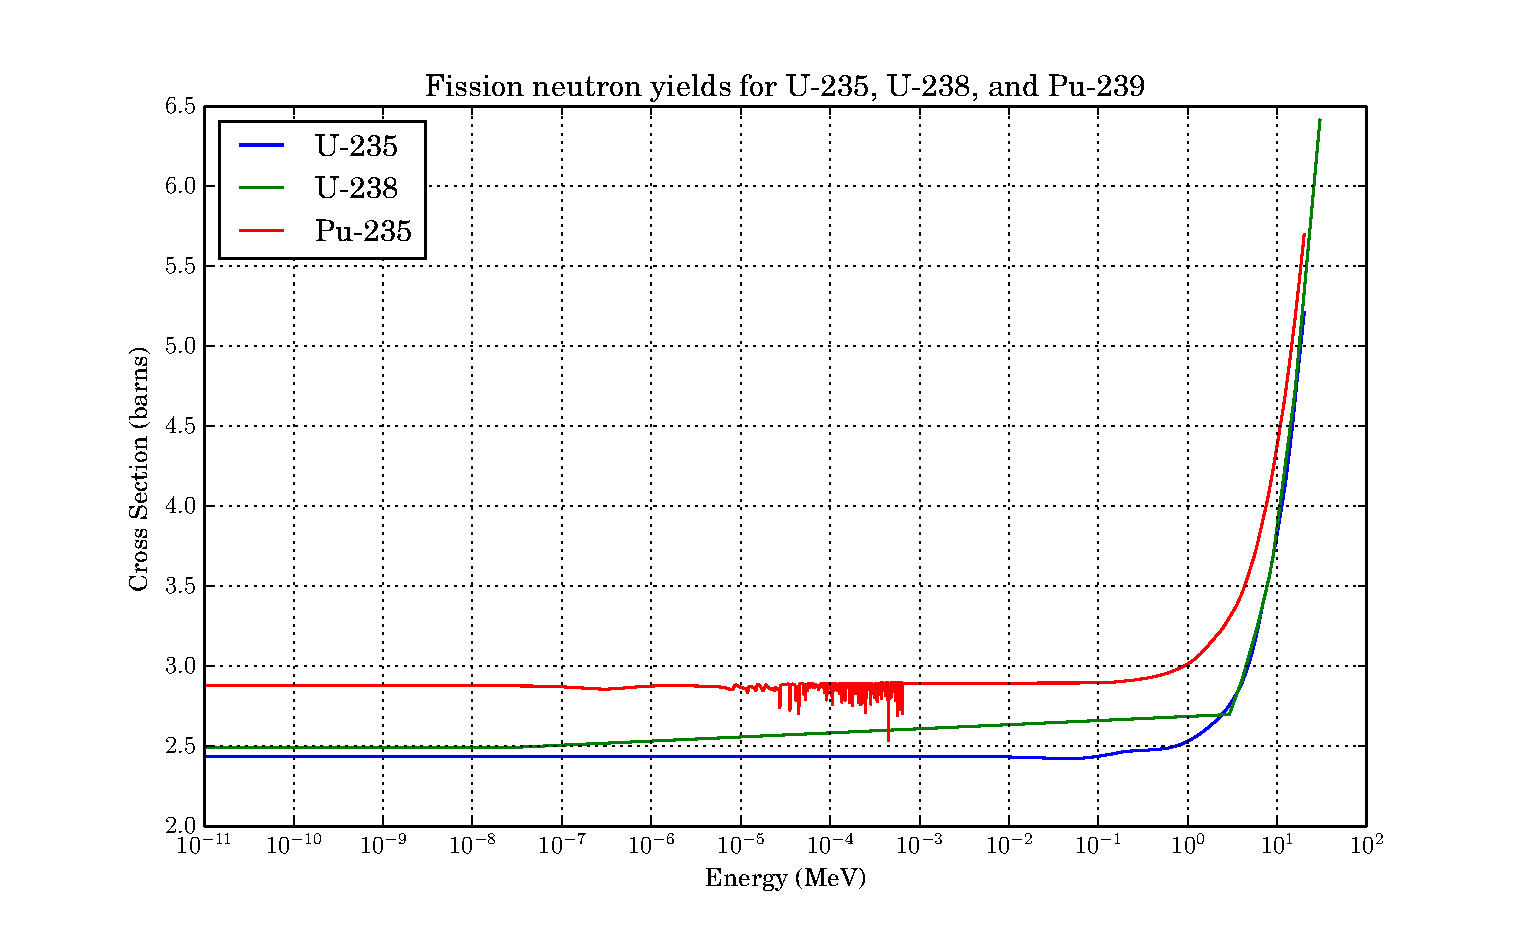
\includegraphics[width=0.8\textwidth]{graphics/nu_compare.eps}
     \caption{Total fission yield, $\nu_\mathrm{T}$, for uranium-235, uranium-238, and plutonium-239.}
\end{figure}

\begin{figure}[h!]
  \label{xs_fission_only}
  \centering
    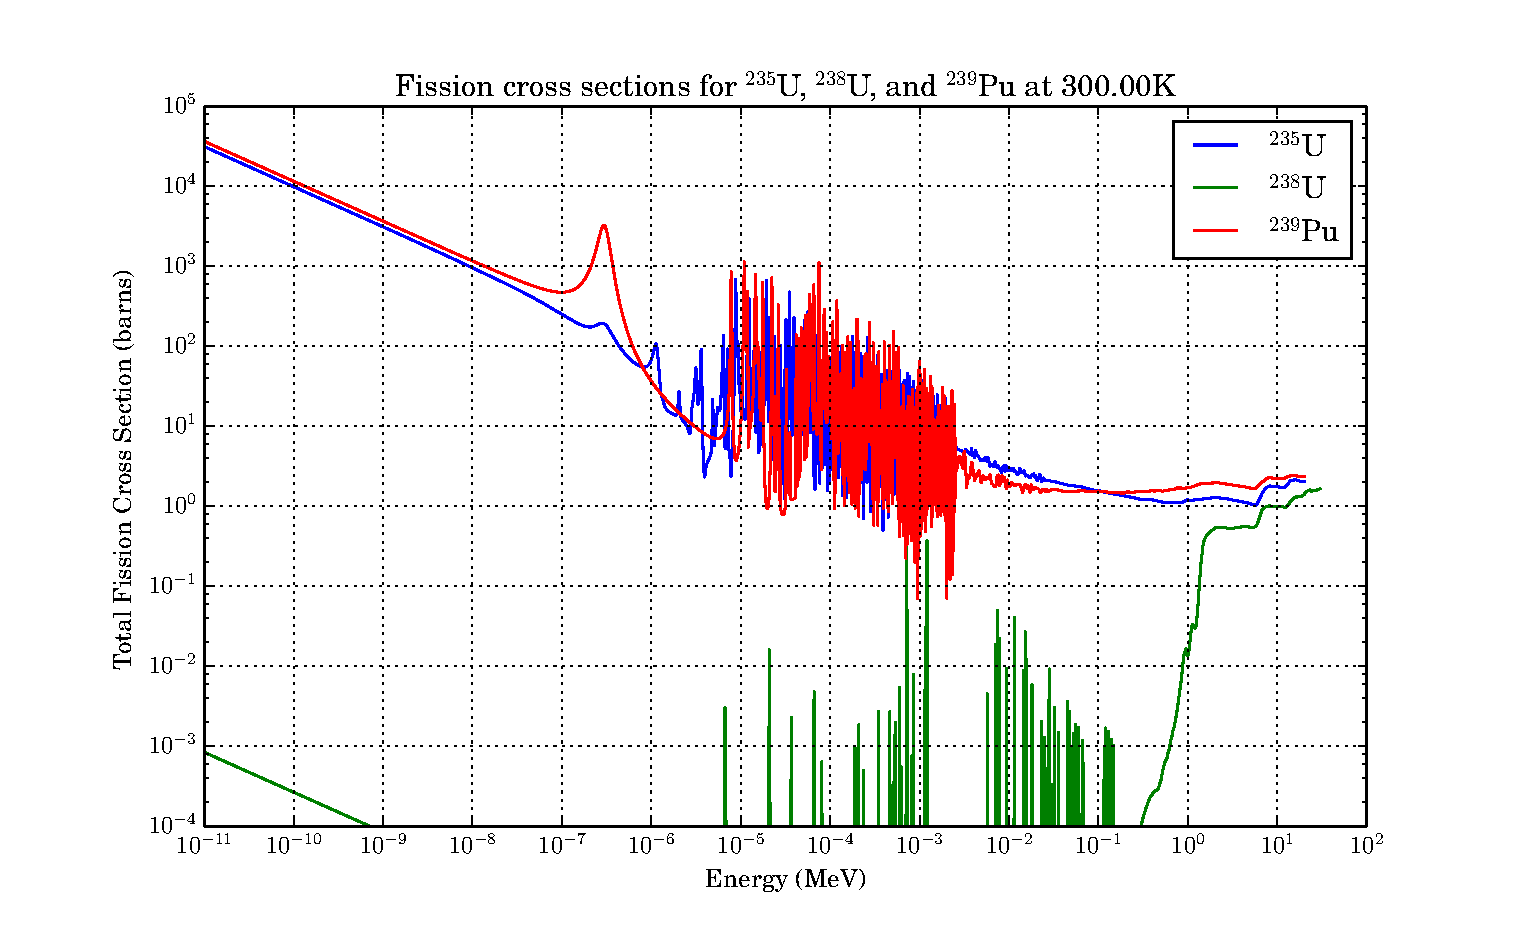
\includegraphics[width=0.8\textwidth]{graphics/xs_fissile.eps}
     \caption{Fission cross sections for uranium-235, uranium-238, and plutonium-239.}
\end{figure}

Figure \ref{nu_compare} shows the energy dependence of the total fission neutron yield, $nu_\mathrm{T}$. It is shown at one temperature since it have very weak temperature dependence.   It can be seen that it is constant until energies in the MeV range, where it increases sharply due to the energy the incident neutron provides being sufficient to eject a bound neutron.  Figure \ref{xs_fission_only} shows the total fission cross sections for two \emph{fissile} isotopes, uranium-235 and plutonium-239, and one \emph{fertile} isotope, uranium-238.  Fissile isotopes are those which neutrons at any energy can induce fission.  The figure shows that uranium-238 has a fission cross section, but it isn't significant until above 1 MeV.  For uranium-238, fission is a threshold reaction.  Simply absorbing a neutron does not provide enough energy to split the nucleus.  Additional energy is required, which can be provided in the form of an incident neutron's kinetic energy.  Uranium-238 isn't fissile, but it can be a significant contributor of fission reactions in reactors where the neutron population is \emph{fast}, i.e. mainly high-energy.  As mentioned before, uranium-238 is considered fertile, which means that it produces a fissile isotope after it absorbs a neutron, and in this case decays to plutonium-239.  

\subsubsection{Other Inelastic Secondary-Producing Reactions}

This category encompasses all the other reactions neutrons undergo.  There are two types, ones that produce secondary neutrons in some amount and those that do not.  Those that do not may still produce other particles, like alpha particles, tritons, protons, et cetera.  Since they do not produce secondary neutrons, however, they are basically equivalent to a disappearance reaction in the scope of neutron transport.  Even though they aren't capture reactions, they can contribute significantly to an isotope's absorption of neutrons.  Figure \ref{xs_e_dependence_li} shows that the (n,$^3$H) in lithium-6 is by far the main component of the total cross section and makes it a very strong absorber of low energy neutrons.  Boron-10 is another great example of this.  Its (n,$\alpha$) reaction has a very high cross section for low energy neutrons, and it is widely used in thermal spectrum reactors in safety and control systems.

Of the reactions that produce secondary neutrons, the (n,2n) reaction is most significant, due to it having the lowest threshold energy.  At higher incident neutron energies, (n,3n) and even (n,4n) can become possible.  Other particle combinations are possible as well, such as (n,n$\alpha$), and these reactions act like an inelastic scatter interaction where the relationship between scattering angle and energy no longer applies due to there being three bodies to distribute energy to instead of only two.

%%%%%%%%%%%%%%%%%%%%%%%%%%%%%%
\subsection{Temperature Effects}

Thus, far there has only been mention of the target nuclide's by how it manifests itself in the 1/$v$ behavior of cross sections at low energy.  Most of the time, it is a good assumption that the thermal motion of the target nuclide is negligible.  Thermal energy is on the order of .01 eV, and this is a good assumption when neutrons are at MeV range energies, but when they scatter and lose energy, they can come near the thermal energy of the material.  When this happens, the target nuclide no longer appears stationary, and assuming that it has zero velocity in scattering calculations is inaccurate.  MCNP sets the threshold at 400kT, which corresponds to about 10 eV for materials at room temperature, above which the target nuclide can be assumed stationary.  Below this threshold, it is important to model thermal effects.  If this wasn't done, a neutron could keep scattering off of zero-energy targets and it's energy could approach zero, which is not physical.  Neutrons can only scatter down to a state where they are in thermal equilibrium with the material they are traveling through.  This creates a ``thermal peak'' at low energies where neutrons collect, especially in materials where the scattering cross section is large and neutrons scatter many times before they are absorbed.

\begin{figure}[h!]
  \label{MB_dist}
  \centering
    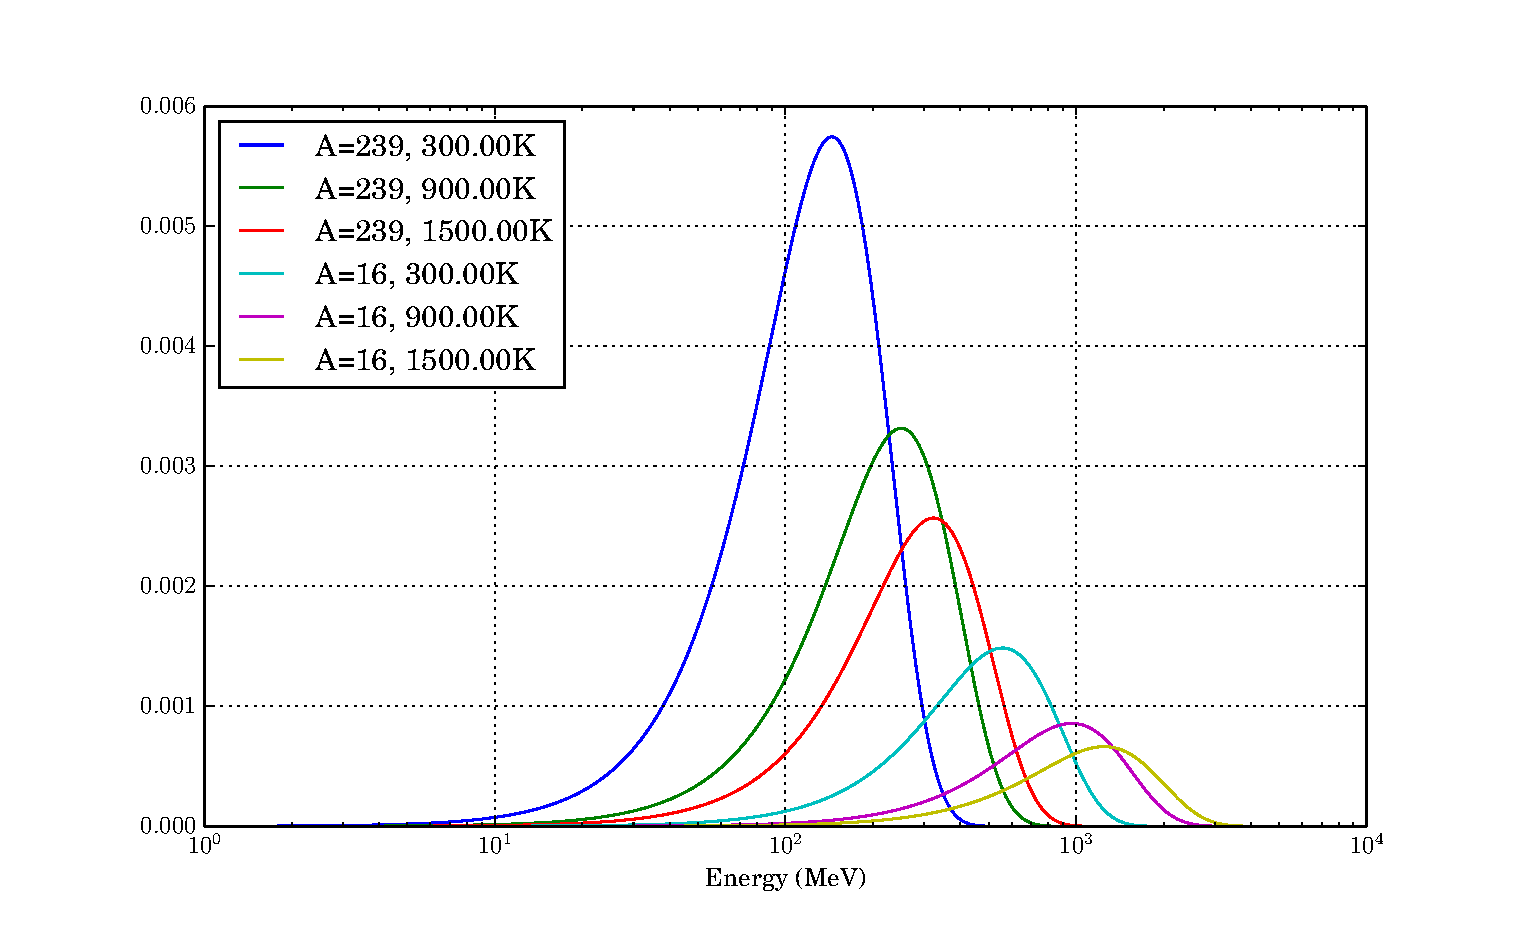
\includegraphics[width=0.8\textwidth]{graphics/MB_dist.eps}
     \caption{Maxwell-Boltzmann distribution for velocity for heavy and light nuclides at different temperatures.}
\end{figure}


\subsubsection{Doppler Effect}


The other effect that thermal motion has is the \emph{Doppler effect}.  This is where resonances are broadened as temperature increases due to the thermal distribution becoming wider, as shown in Figures \ref{MB_dist} and \ref{xs_pu_broaden}.  The effects is also known as \emph{Doppler broadening} for this reason.  Note that the effect is much more pronounced for light nuclei. MORE.  

\begin{figure}[h!]
  \label{xs_pu_broaden}
  \centering
    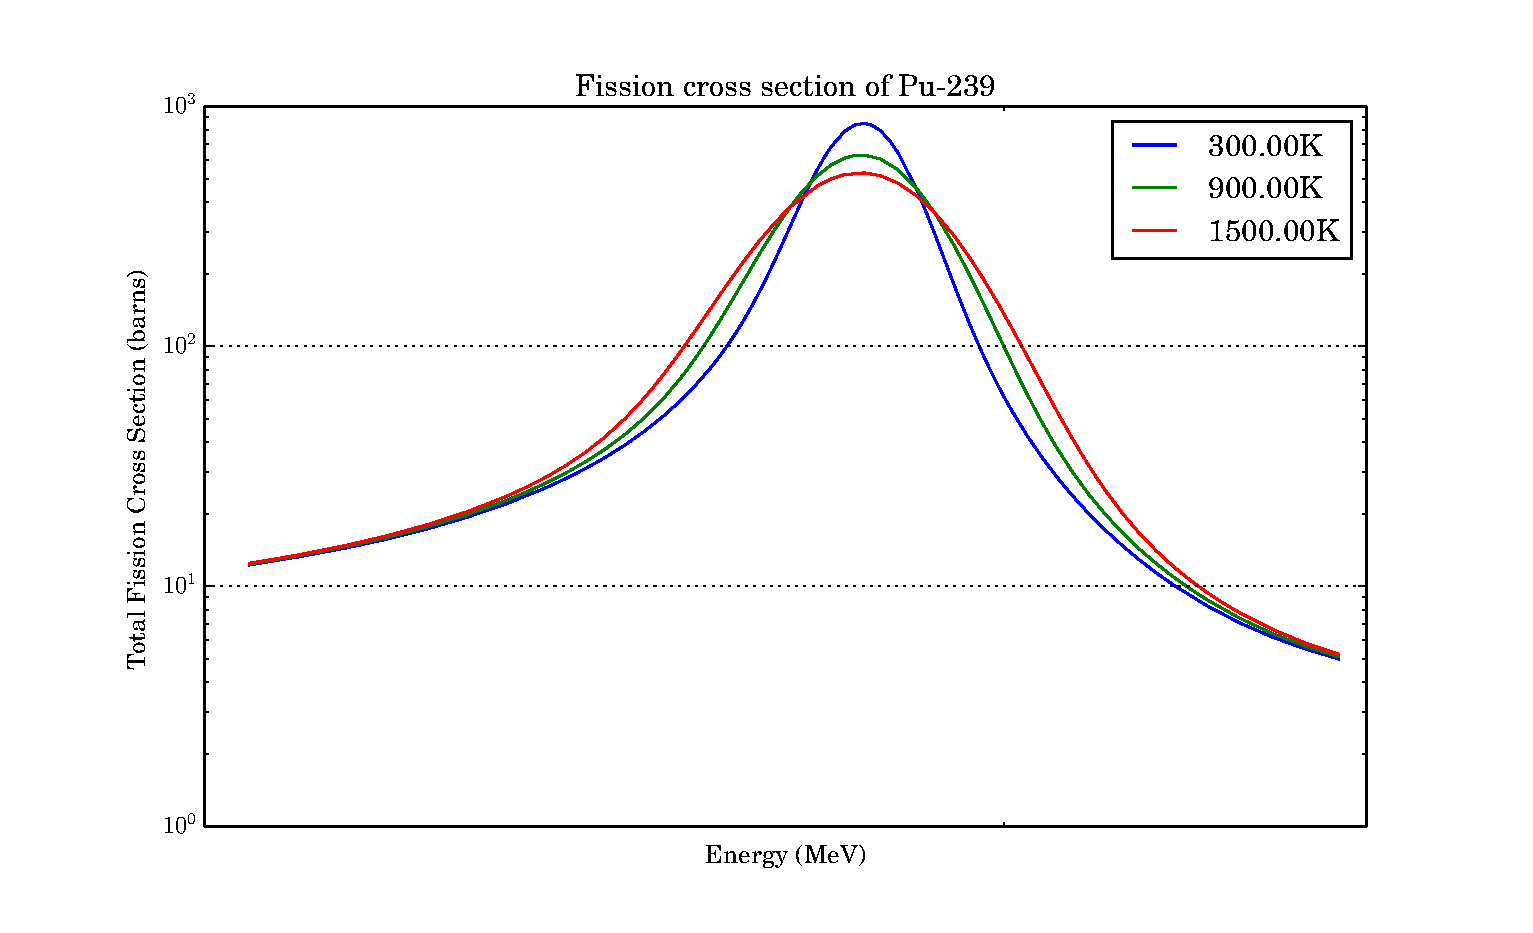
\includegraphics[width=0.8\textwidth]{graphics/xs_pu_broaden.eps}
     \caption{Doppler broadening of the 1eV fission resonance in Pu-239.}
\end{figure}

At 0K, resonances are very sharp and can be treated as delta functions.  To make the assumption that the target is at rest, the thermal distribution must be convolved with the cross section to order to account for the different speeds the targets are moving.  This is especially significant at resonances since slight movements in velocity can produce very large differences in cross section.  The exact method for doing this is shown in \eqref{broaden}\cite{broaden_text}.

\begin{equation}
\begin{split}
such\\
equation
 \end{split}
\label{broaden}
\end{equation}


%%%%%%%%%%%%%%%%%%%%%%%%%%%%%%
\subsection{Neutron Transport}

NTE

\begin{equation}
\end{equation}

\subsection{Discrete Methods}

Diffusion, SN

drawbacks, limitations

\subsection{Monte Carlo}

instead of the neutron population being continuous and the spatial and energy dimensions discretized (and integrating along them), we make the population discrete (and integrate over it) and leave the other dimensions continuous! 

equations and derivations and such

scaling

advantages

drawbacks and limitations

sampling schemes

\subsubsection{Free Gas Treatment}

%%%%%%%%%%%%%%%%%%%%%%%%%%%%%%

\section{GPUs}

Part of the reason GPUs are able to perform efficiently is do to their reliance on single instruction, multiple data (SIMD) execution.  This execution method uses the same instructions carried out over multiple pieces of data at the same time.  This reduces the amount of power used in control and therefore more math can be done per watt [citation definitely needed].  The GPU programming model abstracts SIMD execution by using threads, which can be thought of in the traditional sense . There are some tradeoffs, however, including limited on-board memory (currently 12 GB), limited cache and control space, and requiring data parallelism for full utilization.

Since all threads in a GPU thread block must execute the same instructions, having conditional statements based on random numbers can cause threads to be serialized, leading to resource under-utilization.  For example, in particle transport where a particle history is assigned to each thread, thread divergence mainly arises through particles undergoing different reactions based on the results of cross-section sampling.  Also, GPUs have even higher global memory latency than CPUs, up to 800 clock cycles on older cards, compared to about 50 cycles on a typical CPU.  It is also important to remember than GPUs are clocked much slower than CPUs, so the memory latency performance issue is even greater [5, 7]. 

another brief introduction.  

advantages

pitfalls, weaknesses

\subsection{Supercomputing}

how and why they came to be used for supercomputing.

\subsection{Architecture}

SIMD, threads

\subsection{Memory}

speed, levels, etc.  limitations 

\subsection{CUDA}

kernels

%%%%%%%%%%%%%%%%%%%%%%%%%%%%%%

\section{Previous Works}

talk about the work that other people did

\section{Preliminary Studies}

all my prelim work to motivate this project

\subsection{2D Scattering Game}


\subsection{Ray Tracing with OptiX}

%%%%%%%%%%%%%%%%%%%%%%%%%%%%%%

\section{Scope in Detail}


